\documentclass[aspectratio=169]{beamer}
\usepackage{amsmath}
\usepackage{amssymb}
\usepackage{tikz}
\usepackage{fancyvrb}
\usepackage{xcolor}
\title{Symbolic Execution with Angr\\RPISEC}
\date{December 6, 2019}
\author{Avi Weinstock (\Verb|aweinstock|), Luke Biery (\Verb|tiecoon|)}

\definecolor{rpisecbgcolor}{RGB}{21, 24, 32} % 151820
\definecolor{cybercyan}{RGB}{42, 171, 219} % 2aabdb
\definecolor{cybergreen}{RGB}{106, 220, 169} % 6adca9
\definecolor{cyberpink}{RGB}{248, 106, 140} % f86a8c

\setbeamercolor{normal text}{fg=white}
\setbeamercolor{frametitle}{fg=cybercyan}
\setbeamercolor{title}{fg=cybercyan}
\setbeamercolor{structure}{fg=cybercyan}

%>>> [0x15,0x18,0x20]
%[21, 24, 32]
% convert rpisec_background.png -alpha set -fill '#15182080' -draw 'rectangle 0 0 1090 1216' rpisec_background2.png
% convert probable_prime.png -alpha set -fill '#151820c0' -draw 'rectangle 0 0 414 836' probable_prime2.png
\usebackgroundtemplate{
\colorbox{rpisecbgcolor}{\raisebox{1pt}[\paperheight][\depth]{\hspace{0.6\paperwidth}
%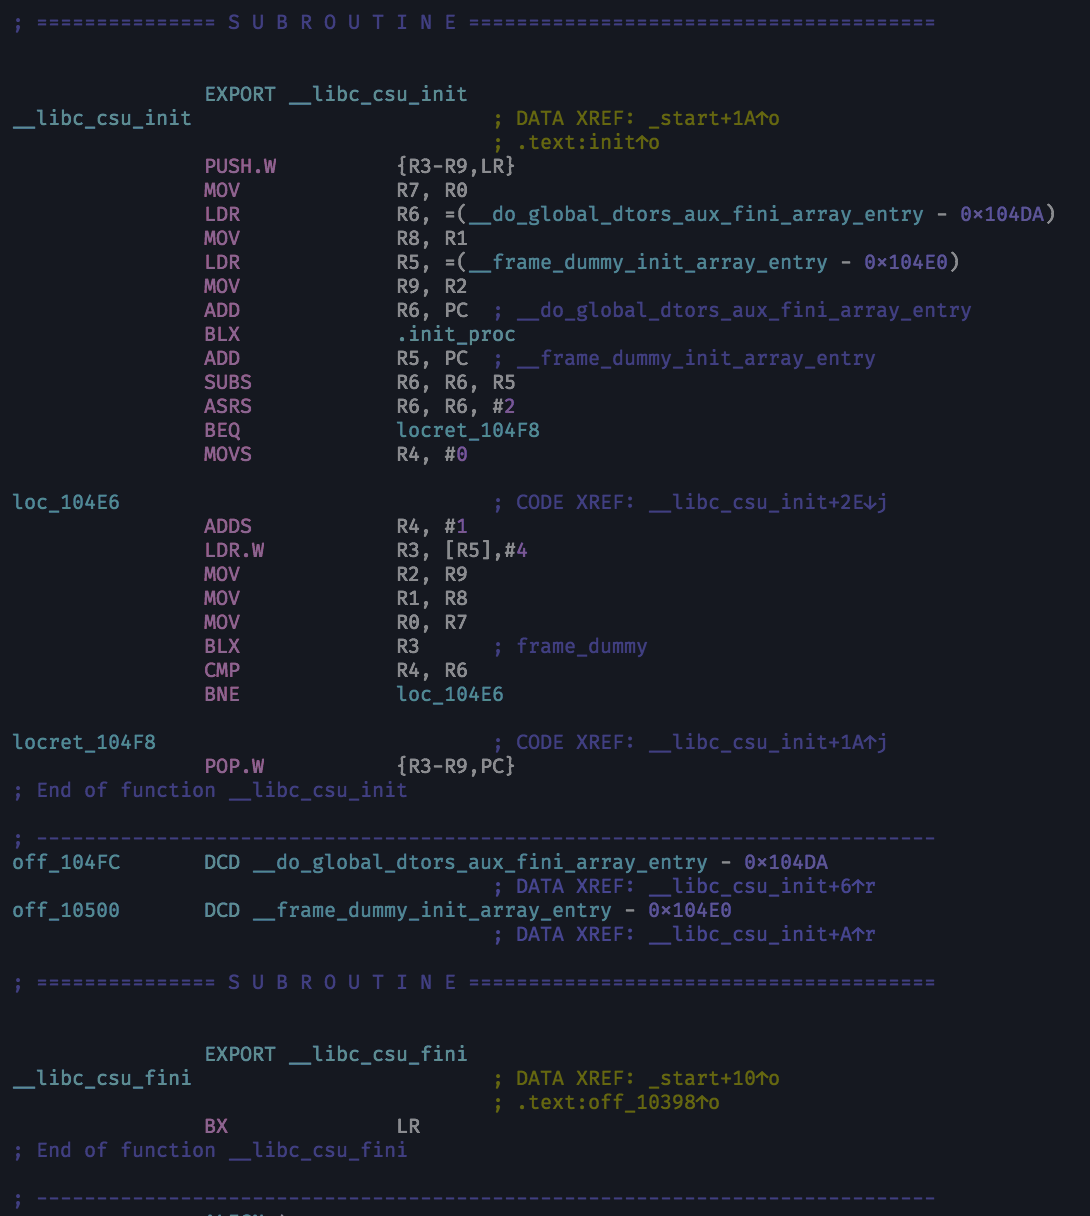
\includegraphics[width=0.4\paperwidth, height=\paperheight]{rpisec_background2.png}
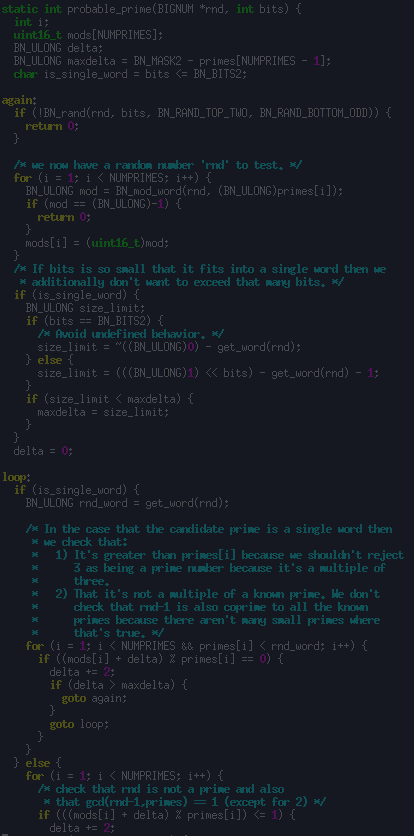
\includegraphics[width=0.4\paperwidth, height=\paperheight]{../rsa_2019_10_29/probable_prime2.png}
}}
}

\newcommand{\SlideWithCenteredText}[1]{
  \begin{frame}
  \vfill
  \centering
  \begin{beamercolorbox}[sep=8pt,center,shadow=true,rounded=true]{title}
    \usebeamerfont{title}#1\par%
  \end{beamercolorbox}
  \vfill
  \end{frame}
}

\newcommand{\questionsslide}[1]{\SlideWithCenteredText{Any questions#1?}}

% https://tex.stackexchange.com/questions/178800/creating-sections-each-with-title-pages-in-beamers-slides
\AtBeginSection[]{
\SlideWithCenteredText{\insertsectionhead}
}



\begin{document}
\maketitle

\begin{frame}[fragile]
\frametitle{Overview}
\begin{itemize}
\item What is Symbolic Execution? What techniques does it compete with?
\item How symbolic execution works (theory)
\item How symbolic execution works (Angr commands)
\item Solving MBE lab1A with Angr
\end{itemize}
\end{frame}

\section{Background - What it is and what is the problem space?}
\begin{frame}[fragile]
\frametitle{What is Symbolic Execution?}
\begin{itemize}
\item Executes a program with symbolic data (usually input)
\item Essentially runs a program on "all possible inputs" at once
\item Instead of having concrete data in each variable/address, \\variables/addresses store trees of what to do with the input
\end{itemize}
\end{frame}

\begin{frame}[fragile]
\frametitle{What problems does Symbolic Execution solve?}
\begin{itemize}
\item What input to provide to reach/avoid a specific line of code?
\item How is a value deep in the program affected by some specific input?
\item Do any inputs lead to any crash?
\item On a crashing input, what registers are controlled by the input?
\end{itemize}
\end{frame}

\begin{frame}[fragile]
\frametitle{Symbolic Execution vs Fuzzing}
\begin{tabular}{c|c}
Symbolic Execution & Fuzzing\\\hline
\textcolor{green}{+ Explores all inputs} & \textcolor{red}{- Only explores random inputs}\\
\textcolor{green}{+ Very detailed output} & \textcolor{red}{- Only learn crash vs non-crash}\\
\textcolor{red}{- Uses more memory/time} & \textcolor{green}{+ Uses around as much memory/time as target program}
\end{tabular}
\begin{itemize}
\item Symbolic execution can the path \verb|if(input == 0xdeadbeefdeadbeef) { ... }|
\item Even coverage-guided fuzzing will only find it $\frac{1}{2^{64}}$ of the time\footnote{Unless the compare is digit-by-digit}
\end{itemize}
%TODO: more comparisons/columns? emphasize that "all inputs" means that symexec can find constant-time comparisons against a giant constant, unlike coverage-guided?
\end{frame}

\questionsslide{ so far}
\section{How symbolic execution works in general}

\begin{frame}[fragile]
\frametitle{Setting up a state for symbolic execution}
\begin{itemize}
\item \begin{Verbatim}[fontsize=\scriptsize, frame=single]
import z3
registers = ['eax', 'ebx', 'ecx', 'edx', 'ebp', 'esp'] # and so on
symstate = {reg: z3.BitVec(reg, 32) for reg in registers}
symstate['memory'] = z3.Array('memory', z3.BitVecSort(32), z3.BitVecSort(8))
\end{Verbatim}
\item Note that the z3 variable \verb|eax| in the model will be the starting value of \verb|eax|
\item \verb|symstate['eax']| will be mutated throughout the computation, and will contain an expression corresponding to the ending value of \verb|eax|
\end{itemize}
\end{frame}

\begin{frame}[fragile]
\frametitle{\texttt{z3.Array} vs dict of \texttt{z3.BitVec} for representing memory}
\begin{itemize}
\item \verb|memory = z3.Array('memory', z3.BitVecSort(32), z3.BitVecSort(8))| symbolically represents an array of $2^{32}$ bytes (around 4GB)
\item \verb|z3.Store(memory, index, value)| represents a modified memory (with \verb|value| written to \verb|index|), even with \textit{symbolic} \verb|index| and \verb|value|
\item \verb|memory[index]| represents a read from memory, even if \verb|index| is symbolic
\item \verb|memory = {i: z3.BitVec('mem[{i}]'.format(i=i), 8) for i in idxs}| only allows concrete indices, while still allowing symbolic values, and is more efficient when we know we won't have symbolic-indexed reads/writes
\end{itemize}
\end{frame}

\begin{frame}[fragile]
\frametitle{Symbolically executing branch-free code}
\begin{itemize}
\item Translate arithmetic, indexing, etc into SMT constraints
\item Angr internally uses VEX for this instead of translating x86 directly
\end{itemize}
\begin{minipage}{0.3\textwidth}
\begin{Verbatim}[fontsize=\scriptsize, frame=single]
mov eax, ebx
\end{Verbatim}
\end{minipage}
\begin{minipage}{0.68\textwidth}
\begin{Verbatim}[fontsize=\scriptsize, frame=single]
symstate['eax'] = symstate['ebx']
\end{Verbatim}
\end{minipage}

\begin{minipage}{0.3\textwidth}
\begin{Verbatim}[fontsize=\scriptsize, frame=single]
add ecx, edx
\end{Verbatim}
\end{minipage}
\begin{minipage}{0.68\textwidth}
\begin{Verbatim}[fontsize=\scriptsize, frame=single]
symstate['ecx'] += symstate['edx']
\end{Verbatim}
\end{minipage}

\begin{minipage}{0.3\textwidth}
\begin{Verbatim}[fontsize=\scriptsize, frame=single]
mov byte [esp+0x10], al
\end{Verbatim}
\end{minipage}
\begin{minipage}{0.68\textwidth}
\begin{Verbatim}[fontsize=\scriptsize, frame=single]
esp_10 = symstate['esp']+0x10
al = z3.Extract(7, 0, symstate['eax'])
symstate['memory'] = z3.Store(symstate['memory'], esp_10, al)
\end{Verbatim}
\end{minipage}

\begin{minipage}{0.3\textwidth}
\begin{Verbatim}[fontsize=\scriptsize, frame=single]
movsx eax, byte [eax]
\end{Verbatim}
\end{minipage}
\begin{minipage}{0.68\textwidth}
\begin{Verbatim}[fontsize=\scriptsize, frame=single]
star_eax = z3.Select(symstate['memory'], eax)
symstate['eax'] = z3.SignExt(24, star_eax)
\end{Verbatim}
\end{minipage}
\end{frame}

\begin{frame}[fragile]
\frametitle{Handling symbolic reads with \texttt{z3.Array} vs \texttt{z3.BitVec}}
\begin{minipage}{0.46\textwidth}
C:
\begin{Verbatim}[fontsize=\scriptsize, frame=single]
tmp = username[i];
tmp ^= serial;
\end{Verbatim}
Assembly:
\begin{Verbatim}[fontsize=\scriptsize, frame=single]
0x08048aee      mov edx, dword [local_14h]
0x08048af1      mov eax, dword [arg_8h]
0x08048af4      add eax, edx
0x08048af6      movzx eax, byte [eax]
0x08048af9      movsx eax, al
0x08048afc      xor eax, dword [local_10h]
\end{Verbatim}
\end{minipage}
\begin{minipage}{0.53\textwidth}
List of \verb|z3.BitVec|:
\begin{Verbatim}[fontsize=\scriptsize, frame=single]
eax = z3.SignExt(24, sym_username[local_14h])
eax ^= local_10h
\end{Verbatim}
\verb|z3.Array|:
\begin{Verbatim}[fontsize=\scriptsize, frame=single]
local_14 = symstate['esp']+0x14 # &i
symstate['edx'] = symstate['memory'][local_14]
arg_8 = symstate['ebp']+0x8 # &username
symstate['eax'] = symstate['memory'][arg_8]
symstate['eax'] += symstate['edx']
symstate['eax'] = z3.ZeroExt(24,symstate['eax'])
al = z3.Extract(7, 0, symstate['eax'])
symstate['eax'] = z3.SignExt(24, al)
local_10 = symstate['esp']+0x10 # &serial
symstate['eax'] ^= symstate['memory'][local_10]
\end{Verbatim}
\end{minipage}
\end{frame}

\questionsslide{ so far}

\begin{frame}[fragile]
\frametitle{Symbolically executing branchs - Graphically}
\begin{minipage}{0.25\textwidth}
\begin{Verbatim}[fontsize=\scriptsize, frame=single]
int f(int x, int y) {
    if (x > 3) {
        x += 1;
    } else {
        y = 2*y+3;
    }
    if(y != 0) {
        x /= y;
    } else {
        x *= 2;
    }
    return x + y;
}
\end{Verbatim}
\end{minipage}
\begin{minipage}{0.6\textwidth}
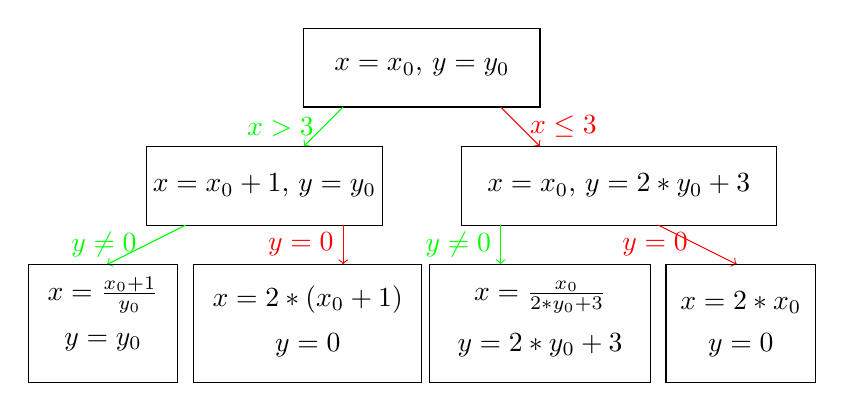
\begin{tikzpicture}
\draw (-1.5,5) rectangle node{$x = x_0$, $y = y_0$} (1.5,4);

\draw[green, ->] (-1,4) -- node[left]{$x > 3$} (-1.5, 3.5); 
\draw (-3.5,3.5) rectangle node{$x = x_0+1$, $y = y_0$} (-0.5,2.5);
\draw[red, ->] (1,4) -- node[right]{$x \le 3$} (1.5, 3.5); 
\draw (0.5,3.5) rectangle node{$x = x_0$, $y = 2*y_0+3$} (4.5,2.5);

\draw[green, ->] (-3,2.5) -- node[left]{$y \neq 0$} (-4, 2); 
\draw (-5, 2) rectangle node[above]{$x = \frac{x_0+1}{y_0}$} node[below]{$y = y_0$} (-3.1, 0.5);
\draw[red, ->] (-1,2.5) -- node[left]{$y = 0$} (-1, 2); 
\draw (-2.9, 2) rectangle node[above]{$x = 2*(x_0+1)$} node[below]{$y = 0$} (-0, 0.5);

\draw[green, ->] (1,2.5) -- node[left]{$y \neq 0$} (1, 2); 
\draw (2.9, 2) rectangle node[above]{$x = \frac{x_0}{2*y_0+3}$} node[below]{$y = 2*y_0+3$} (0.1, 0.5);
\draw[red, ->] (3,2.5) -- node[left]{$y = 0$} (4, 2); 
\draw (5, 2) rectangle node[above]{$x = 2*x_0$} node[below]{$y = 0$} (3.1, 0.5);
\end{tikzpicture}
\end{minipage}
\end{frame}

\begin{frame}[fragile]
\frametitle{Symbolically executing branchs - Programmatically}
\begin{minipage}{0.25\textwidth}
\begin{Verbatim}[fontsize=\scriptsize, frame=single]
int f(int x, int y) {
    if (x > 3) {
        x += 1;
    } else {
        y = 2*y+3;
    }
    if(y != 0) {
        x /= y;
    } else {
        x *= 2;
    }
    return x + y;
}
\end{Verbatim}
\end{minipage}
\begin{minipage}{0.74\textwidth}
\begin{Verbatim}[fontsize=\scriptsize, frame=single]
import z3
x0, y0 = z3.Ints('x0 y0')
states, newstates = [(x0, y0, z3.Solver())], []
for (x, y, s) in states:
  t = s.__deepcopy__()
  s.add(x > 3); newstates.append((x+1, y, s))
  t.add(z3.Not(x > 3)); newstates.append((x, 2*y+3, t))

states, newstates = newstates, []
for (x, y, s) in states:
  t = s.__deepcopy__()
  s.add(y != 0); newstates.append((x/y, y, s))
  t.add(z3.Not(y != 0)); newstates.append((2*x, y, t))

for (x, y, s) in newstates:
  print('x: %r; y: %r; s: %r; check: %r' % (x, y, s, s.check()))
  if s.check() == z3.sat:
    m = s.model()
    print('m: %r; x: %r; y: %r' % (m, m.evaluate(x), m.evaluate(y)))
    print('-'*5)
\end{Verbatim}
\end{minipage}
\end{frame}

\begin{frame}[fragile]
\frametitle{Symbolically executing loops}
\begin{minipage}{0.35\textwidth}
\begin{Verbatim}[fontsize=\scriptsize, frame=single]
void memcpy(
    char *dest,
    const char *src,
    size_t n) {
    for(size_t i=0; i<n; i++) {
        dest[i] = src[i];
    }
}
\end{Verbatim}
\end{minipage}
\begin{minipage}{0.6\textwidth}
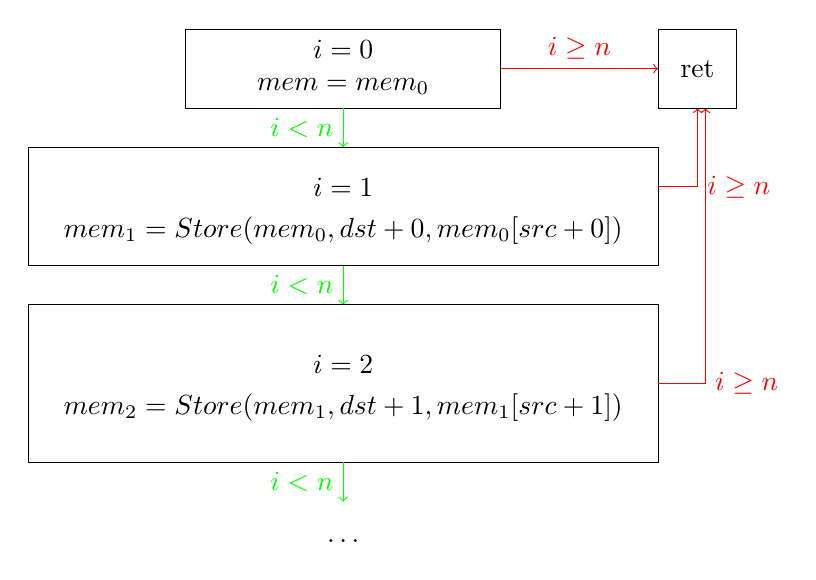
\begin{tikzpicture}
\draw (0,5) rectangle node[above]{$i=0$} node[below]{$mem = mem_0$} (4,4);
\draw[green, ->] (2,4) -- node[left]{$i < n$} (2, 3.5); 
\draw[red, ->] (4,4.5) -- node[above]{$i \ge n$} (6, 4.5); 

\draw (-2,3.5) rectangle node[above]{$i=1$} node[below]{$mem_1 = Store(mem_0, dst+0, mem_0[src+0])$} (6,2);
\draw[green, ->] (2, 2) -- node[left]{$i < n$} (2, 1.5); 
\draw[red, ->] (6,3) -| node[right]{$i \ge n$} (6.5, 4); 

\draw (-2,1.5) rectangle node[above]{$i=2$} node[below]{$mem_2 = Store(mem_1, dst+1, mem_1[src+1])$} (6,-0.5);
\draw[green, ->] (2, -0.5) -- node[left]{$i < n$} (2, -1); 
\draw (2, -1.5) node{$\hdots$};
\draw[red, ->] (6,0.5) -| node[right]{$i \ge n$} (6.6, 4); 

\draw (6, 5) rectangle node{ret} (7, 4);
\end{tikzpicture}
\end{minipage}
\end{frame}

\questionsslide{ so far}
\section{How to use Angr for symbolic execution}

\begin{frame}[fragile]
\frametitle{Angr}
\begin{itemize}
\item A very useful tool for RE made by shellphish and now maintained by SEFCOM at Arizona State University as well
\item Originally made for DARPA’s cyber grand challenge.
\item A very strong framework for emulation allowing symbolic values.
\end{itemize}
\end{frame}

\begin{frame}[fragile]
\frametitle{Angr - The basics}
\begin{itemize}
\item It is written almost entirely in python and as such currently only has python bindings.
\item Installation
\begin{itemize}
\item Has a couple dependencies that may conflict with other packages so it is recommended to use python virtual environments.
\item \verb|$ pip install --user angr|
\item Now you can just import angr in any python interpreter
\end{itemize}
\end{itemize}
\end{frame}

\begin{frame}[fragile]
\frametitle{Angr - Writing a script}
\begin{itemize}
\item The basic block in angr is a project
\item It is how you tell angr what file to load
\item Can be used to obtain a bunch of metadata as well about the file
\begin{itemize}
\item \verb|project = angr.Project("./binary")|
\end{itemize}
\end{itemize}
\end{frame}

\begin{frame}[fragile]
\frametitle{Angr - Writing a script}
\begin{itemize}
\item Accessing everything else will be done through factory
\begin{itemize}
\item \verb|project.factory|
\end{itemize}
\item Next you will have to tell angr where it should start
\item Most of the time you want this to be \verb|entry_state()|
\begin{itemize}
\item This will setup everything as it would be at the entry point if you ran the binary
\item This is where you would tell it if you wanted a special stdin or args
\begin{itemize}
\item You can use claripy to make it symbolic
\end{itemize}
\end{itemize}
\end{itemize}
\end{frame}

\begin{frame}[fragile]
\frametitle{Angr - Simulation manager}
\begin{itemize}
\item This will hold all your various states as they are created and abandoned
\begin{itemize}
\item \verb|sm = project.factory.simulation_manager(state)|
\end{itemize}
\item Executing
\begin{itemize}
\item To execute you will normally want to use \verb|.run()| or \verb|.explore()|
\item Explore
\begin{itemize}
\item Allows you to guide execution better and limit computation necessary
\item You can specify find and avoid conditions via addresses or lambda functions
\end{itemize}
\item Run
\begin{itemize}
\item Will just run every state until exhaustion
\item Theoretically tells you all possible outcomes of the program
\item Prone to path explosion
\end{itemize}
\item Many more that are more application specific
\end{itemize}
\end{itemize}
\end{frame}

\begin{frame}[fragile]
\frametitle{Angr - States}
\begin{itemize}
\item States will allow you to introspect, touch or check memory values
\item For now we will only be touching state.posix
\begin{itemize}
\item This allows access to the various posix style file descriptors on supported systems
\item Alot you can do here by using hooks and moving states between stashes
\end{itemize}
\item Stashes
\begin{itemize}
\item Active
\item Deadended
\item Pruned
\item Unconstrained
\item Unsat
\end{itemize}
\end{itemize}
\end{frame}

\begin{frame}[fragile]
\frametitle{Angr - Symbolic Values}
\begin{itemize}
\item Angr uses a library called claripy which is their wrapper for constraint solvers
\item Used in place of direct Z3 calls so it is portable between different backends
\item Shouldn't need to touch anything besides
\begin{itemize}
\item BV - bitvector
\item FP - floating point
\item Bool - boolean
\end{itemize}
\item Then just like in Z3 you can perform math with these, however to combine them one after another you need to use Concat()
\item NOTE: The default python \verb|>|, \verb|<|, \verb|>=|, and \verb|<=| are unsigned in Claripy. This is different than their behavior in Z3, because it seems more natural in binary analysis.
\end{itemize}
\end{frame}

\section{Example: Fairgame RE400 with Angr}
\begin{frame}[fragile]
\frametitle{Fairgame RE400 Ghidra decompilation}
\begin{minipage}{0.5\textwidth}
\begin{Verbatim}[frame=single, fontsize=\tiny]
int main () {
  puts("[+] Welcome to the REvision 400 lock firmware.");
  uStack288 = 0x1008b1;
  puts("[!] Please enter the serial:");
  uStack288 = 0x1008cc;
  fgets(&local_118,0xfe,stdin);
  uStack288 = 0x1008db;
  sVar2 = strlen(&local_118);
  *(&uStack288 + sVar2 + 7) = 0;
  uStack288 = 0x1008f6;
  mangle(&local_118);
  uStack288 = 0x100911;
  iVar1 = memcmp(&local_118,expect,0xfe);
  if (iVar1 == 0) {
    uStack288 = 0x100921;
    puts("[+] REvision 400 lock firmware unlocked.");
  }
  else {
    uStack288 = 0x10092f;
    puts("[-] Invalid serial.");
  }
  if (local_10 != *(in_FS_OFFSET + 0x28)) {
                    /* WARNING: Subroutine does not return */
    uStack288 = 0x100948;
    __stack_chk_fail();
  }
  return 0;
}
\end{Verbatim}
\end{minipage}
\begin{minipage}{0.49\textwidth}
\begin{Verbatim}[frame=single, fontsize=\tiny]
void mangle(char *input) {
  int i;
  i = 0;
  while (i < 0xfe) {
    swap(input + i,
         input + *(map + i * 4),
         input + *(map + i * 4),
         i);
    i = i + 1;
  }
  return;
}
\end{Verbatim}
\begin{Verbatim}[frame=single, fontsize=\tiny]
oid swap(char *param_1,char *param_2) {
  char cVar1;
  
  cVar1 = *param_1;
  *param_1 = *param_2;
  *param_2 = cVar1;
  return;
}
\end{Verbatim}
\end{minipage}
\end{frame}

\begin{frame}[fragile]
\frametitle{Fairgame RE400 script and output}
\begin{minipage}{0.55\textwidth}
Script:
\begin{Verbatim}[frame=single, fontsize=\tiny]
import angr
import claripy

p = angr.Project("./re400")

for j in range(0xFF):
    # make a symbolic list of j bytes
    flag_chars = [claripy.BVS("serial_%d" % i, 8) for i in range(j)]
    # combine them all
    flag = claripy.Concat(*flag_chars)

    # tell angr to start at entry
    init = p.factory.entry_state(stdin=flag)

    sm = p.factory.simulation_manager(init)

    # find a state with "unlocked" in stdout
    sm.explore(find=lambda s: b"unlocked" in s.posix.dumps(1))

    # try next length if not found
    if len(sm.found) == 0:
        continue
    print('Good length: %d' % (j,))

    print(sm)
    for i in sm.found:
        print(i.posix.dumps(1))
        print(i.posix.dumps(0))
    break
\end{Verbatim}
\end{minipage}
\begin{minipage}{0.44\textwidth}
Redacted output:
\begin{Verbatim}[frame=single, fontsize=\tiny]
Good length: 25
<SimulationManager with 1 active, 1 found>
b'[+] Welcome to the REvision 400 lock firmware.\n
[!] Please enter the serial:\n
[+] REvision 400 lock firmware unlocked.\n'
b'flag{__________________}\xff'
python script.py  154.01s user 2.08s system
102% cpu 2:31.85 total
\end{Verbatim}
\end{minipage}
\end{frame}

\questionsslide{ overall}

\begin{frame}[fragile]
\frametitle{Winter challenge announcement}
\begin{itemize}
\item \verb|root-me.org| has a decent set of challenges in many categories \{pwn, crypto, web, misc\}
\item We'll be providing prizes (book orders on No Starch Press) based on completion over the winter break
\item Details TBD, check for email on the RPISEC mailing list
\end{itemize}
\end{frame}

\begin{frame}[fragile]
\frametitle{Resources}
\begin{itemize}
\item \verb|https://github.com/angr/|
\item \verb|https://github.com/Z3Prover/z3/|
\item \verb|https://github.com/RPISEC/MBE|
\end{itemize}
\end{frame}
\end{document}
